\documentclass[tikz]{standalone}
\usepackage{xcolor}
\usetikzlibrary{arrows,positioning,quotes,backgrounds,arrows.meta,bending,positioning,shapes,shapes.geometric}
\begin{document}
\pgfdeclarelayer{background}
\pgfsetlayers{background,main}
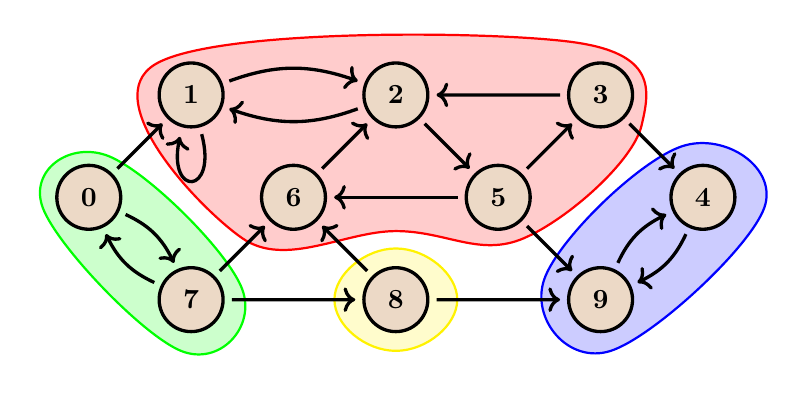
\begin{tikzpicture}
	[scale=1.3,very thick,every circle node/.style={draw,inner sep=0.18cm,outer sep=1.1mm,fill=brown!30}, every path/.style={->}]

	%\draw[help lines] (-1,-2) grid (7,2);
	\node[circle] (0) at (0,0) {\textbf0};
	\node[circle] (1) at (1,1) {\textbf1};
	\node[circle] (2) at (3,1) {\textbf2};
	\node[circle] (3) at (5,1) {\textbf3};
	\node[circle] (4) at (6,0) {\textbf4};
	\node[circle] (5) at (4,0) {\textbf5};
	\node[circle] (6) at (2,0) {\textbf6};
	\node[circle] (7) at (1,-1) {\textbf7};
	\node[circle] (8) at (3,-1) {\textbf8};
	\node[circle] (9) at (5,-1) {\textbf9};

	\path (0) edge (1);
	\path (0) edge[bend left=20] (7);
    \path (1) edge[loop below] (1);
	\path (1) edge[bend left=20] (2);
	\path (2) edge[bend left=20] (1);
	\path (2) edge (5);
	\path (3) edge (2);
	\path (3) edge (4);
	\path (4) edge[bend left=20] (9);
	\path (5) edge (3);
	\path (5) edge (6);
	\path (5) edge (9);
	\path (6) edge (2);
	\path (7) edge[bend left=20] (0);
	\path (7) edge (6);
	\path (7) edge (8);
	\path (8) edge (6);
	\path (8) edge (9);
	\path (9) edge[bend left=20] (4);

	\begin{pgfonlayer}{background}
		\draw[thick, red, fill=red!20!white] plot [smooth cycle,tension=0.65] coordinates{(0.65,1.3)(4.7,1.52)(5.4,0.7)(4.25,-.4)(3,-.33)(1.5,-.4)};
		\draw[thick, green, fill=green!20!white] plot [smooth cycle,tension=0.7] coordinates{(0.2,0.4)(1.5,-0.9)(.9,-1.5)(-.45,-.1)};
		\draw[thick, blue, fill=blue!20!white] plot [smooth cycle,tension=0.7] coordinates{(5.8,0.5)(4.45,-0.8)(5.1,-1.5)(6.6,-.1)};
		\draw[thick, yellow, fill=yellow!20!white] plot [smooth cycle,tension=0.9] coordinates{(3,-0.5)(3.6,-1)(3,-1.5)(2.4,-1)};
	\end{pgfonlayer}
\end{tikzpicture}

\end{document}
